% -*- mode: LaTeX; coding: utf-8 -*-
\documentclass[12pt]{article}
\usepackage[unicode,colorlinks]{hyperref}
\usepackage[T2A]{fontenc}
\usepackage[utf8]{inputenc}
\usepackage[russian]{babel}
\usepackage{amsmath}
\usepackage{amssymb}
\usepackage{eufrak}
\usepackage{epsfig}
%\usepackage[mathscr]{eucal}
\usepackage{psfrag}
\usepackage{tabularx}
\usepackage{wrapfig}
%\usepackage{eucal}
\usepackage{euscript}
\usepackage{cite}

\usepackage[usenames]{color}
\usepackage{colortbl} 

\definecolor{codegreen}{rgb}{0,0.6,0}
\definecolor{codegray}{rgb}{0.5,0.5,0.5}
\definecolor{codeblack}{rgb}{0.1,0.,0.3}
\definecolor{codeemph}{rgb}{0.5,0.1,0.5}
\definecolor{codepurple}{rgb}{0.58,0,0.82}
\definecolor{backcolour}{rgb}{0.95,0.95,0.92}

\usepackage{listings}\lstset{
	basicstyle=\ttfamily\fontsize{10pt}{10pt}\selectfont\color{codeblack},
  commentstyle=\color{codegray},
	keywordstyle=\tt\bf\color{codeemph},
	belowskip=0pt
    }

\setlength{\topmargin}{-0.5in}
\setlength{\oddsidemargin}{-5.mm}
\setlength{\evensidemargin}{-5.mm}
\setlength{\textwidth}{7.in}
\setlength{\textheight}{9.in}

\def\dfdx#1#2{\frac{\partial #1}{\partial #2}}
\def\hm#1{#1\nobreak\discretionary{}{\hbox{\m@th$#1$}}{}}
\newcommand{\Frac}[2]{\displaystyle\frac{#1}{#2}}

\def\sr#1{{\left<#1\right>}}
\def\m{\mathbf m{}}

\begin{document}
\begin{center}
  \bf\LARGE Кроссплатформенный вьювер qplt \\ с клиент--серверной архитектурой
\end{center}

\tableofcontents

%%%%%%%%%%%%%%%%%%%%%%%%%%%%%%%%%%%%%%%%%%%%%%%%%%%%%%%%%%
\section{Введение}
Вьювер qplt  состоит из клиентской части (интерфейса)
и серверной части (ядра, отвечающего за рендеринг изображения). Интерфейс реализован на языке python3 при помощи библиотеки PyQt5 и является кроссплатформенным.
Возможен запуск интерфейса без ядра, при этом этом связь с ядром осуществляется поверх протокола SSH,
в таком режиме происходит визуализация данных, хранящихся на сервере, без их копирования на клиентскую машину.
За счет минимизации трафика такой режим работы может оказаться быстрее, чем удаленный запуск вьюевра через утилиты ssh -X или vglconnect.
Кроме того, такой режим предъявляет минимальные требования как к клиенту (кроссплатформенность и минимум программных зависимостей),
так и к серверу (минимум программных зависимостей, не требуется настройка vglconnect, переменных окружения DISPLAY и т.д.).


Ядро реализовано на языках C++ и CUDA. Сборка с CUDA (поддержка GPU) опциональна и не является обязательной.
Версия без CUDA использует для распараллеливания технологию OpenMP.
Целевой системой для сборки ядра является OS Linux. Возможна кросскомпиляция под OS Windows при помощи mingw (без CUDA).

При локальном запуске ядро подключается к интерфейсу как разделяемая библиотека (.so или .pyd). Для сборки разеляемой библиотеки применяется пакет SWIG. 
Возможно одновременное подключение к одному интерфейсу одного локального ядра и еще нескольких удаленных ядер через  SSH на различных машинах.
При удаленном подключении qplt передает в ядро параметры отрисовки и принимает картинку. Во всех случаях поверх картинки, сгенерированной ядром,
qplt рисует зарамочное оформление (палитру, оси и подписи к осям).


Для каждого ядра возможна визуализация множества файлов с данными. Во избежание перерасхода памяти в рамках каждого ядра работает свой менеджер памяти,
организующий загрузку данных из файла (по необходимости перед визуализацией) и выгрузку неиспользуемых данных (при превышении лимита выделнной памяти). 
Лимит памяти по умолчанию равен 4Гб и может быть настроен при запуске ядра через аргументы командной строки.

Вьювер qplt реализован как часть библиотеки aiwlib и широко использует C++ классы aiwlib.

Вьювер qplt ориентирован на отображение данных с размерностью $2\div6$, сохраненных в бинарном формате контейнера \verb'aiw::Mesh' библиотеки aiwlib.
В качестве ячейки контейнера может выступать любая POD-структура, определенная пользователем.
Для настройки визуализации необходимо знать типы и расположение (смещения) полей в структуре.
Максимум производительности достигается при визуализации полей типа \verb'float', но возможна визуализация полей
любого встроенного числового типа.

%%%%%%%%%%%%%%%%%%%%%%%%%%%%%%%%%%%%%%%%%%%%%%%%%%%%%%%%%%
\section{Установка и запуск qplt}
\subsection{Получение исходного кода qplt с github вместе с библиотекой aiwlib}
Библиотека aiwlib доступна по адресу \href{https://github.com/aivn/aiwlib}{https://github.com/aivn/aiwlib}
и может быть скачана, например, как
\begin{verbatim}
git clone https://github.com/aivn/aiwlib
\end{verbatim}
После этого без сборки можно использовать клиентскую часть. Сам вьювер расположен в файле \verb'aiwlib/bin/qplt',
для его запуска необходимо либо скопировать (создать символическую ссылку) питоновскую часть библиотеки \verb'aiwlib/python3/aiwlib'
туда, где ее будет видеть интерпретатор \verb'python3' (например, в \verb'/usr/lib/python3' либо в \verb'C:\Python3\Lib'),
либо указать путь к \verb'aiwlib' в конфигурационном файле \verb'~/.qplt'.

Для работы клиентской части необходим python3 с установленными PyQt5 и paramiko. Для установки под Linux можно выполнить команды
\begin{verbatim}
sudo apt install python3-pyqt5 python3-paramiko
\end{verbatim}
Для установки под Windows нужно перейти в директорию, где установлен python3, и выполнить в терминале команды
\begin{verbatim}
wget https://bootstrap.pypa.io/get-pip.py 
python.exe get-pip.py
Scripts\pip.exe install pyqt5
Scripts\pip.exe install paramiko
\end{verbatim}


\subsection{Сборка qplt}
Для сборки qplt необходимы:
\begin{itemize}
\item утилита GNU make;
\item компилятор g++ не ниже версии 4.9;
\item пакет \verb'swig';
\item пакет \verb'python3-dev';
\item опционально, для поддежки GPU ~--- компилятор nvcc.
\end{itemize}
Для сборки необходимо перейти в директорию библиотеки \verb'aiwlib' и выполнить команду
\begin{verbatim}
make python=3 qplt
\end{verbatim}
При возникновении проблем с наличием библиотеки \verb'zlib' ее можно отключить опцией сборки \verb'zlib=off'
или в файле \verb'include/aiwlib/config.mk'

Для сборки с поддежкой GPU необходимо выполнить команду
\begin{verbatim}
make python=3 cuda=on qplt
\end{verbatim}
Путь к компилятору nvcc можно указать при помощи опции \verb'NVCC=...'

Для удаления предыдущей сборки служит команда
\begin{verbatim}
make python=3 clean-qplt
\end{verbatim}
Для выборочного удаления фрагментов, требующих пересборки при помощи nvcc (при включении/выключении поддежки GPU), служит команда
\begin{verbatim}
make python=3 clean-qplt-cu
\end{verbatim}

После этого при выполнении требований предыдущего раздела об обеспечении доступа к каталогу \verb'aiwlib/python3/aiwlib'
вьювер будет работать с использованием локального ядра. При этом установка модуля paramiko не обязательна~--- этот модуль необходим только для удаленного запуска ядра. 


\subsection{Сборка и настройка ядра qplt для работы в режиме сервера}
В качестве сервера qplt может выступать только машина под управлением OS Linux.

Сборка ядра выполняется автоматически при сборке qplt, описанной в предыдущем разделе.
Можно ограничиться только сборкой ядра qplt для работы в режиме сервера.
Для сборки ядра qplt необходимы:
\begin{itemize}
\item утилита GNU make;
\item компилятор g++ не ниже версии 4.9;
\item опционально, для поддежки GPU ~--- компилятор nvcc.
\end{itemize}

Для сборки ядра необходимо выполнить команду
\begin{verbatim}
make bin/qplt-remote
\end{verbatim}
При возникновении проблем с наличием библиотоеки \verb'zlib' ее можно отключить опцией \verb'zlib=off'
или в файле \verb'include/aiwlib/config.mk'

Для сборки ядра с поддежкой GPU необходимо выполнить команду
\begin{verbatim}
make cuda=on bin/qplt-remote
\end{verbatim}
Путь к компилятору nvcc можно указать при помощи опции \verb'NVCC=...'

Для настройки сервера необходимо скопировать (или создать символическую ссылку) файл \verb'bin/qplt-remote' в каталог \verb'~/bin/'.
Кроме того, необходимо настроить вход на сервер по открытому ключу SSH.


\subsection{Бинарная сборка qplt для OS Windows}
Последняя бинарная сборка qplt для OS  Windows доступна по одному из следующих адресов:
\begin{itemize}
\item \href{http://a-iv.ru/qplt/qplt.zip}{https://a-iv.ru/qplt/qplt.zip}
\end{itemize}
После распаковки архива необходимо запускать файл \verb'qplt\qplt.exe'.
Бинарная сборка qplt для OS  Windows обеспечивает локальный и удаленный запуск ядра qplt, но не поддерживает GPU при локальном запуске ядра.

Для самостоятельной кросскомпиляции под Windows дополнительно требуются
\begin{itemize}
\item пакет \verb'wine';
\item пакет \verb'g++-mingw-w64-x86-64'
\end{itemize}

Для кросскомпиляции необходимо выполнить следующие действия:
\begin{enumerate}
\item Запустить \verb'winecfg' и установить версию OS Windows 10.
\item Скачать дистрибутив Python для OS Windows
\begin{verbatim}
wget https://www.python.org/ftp/python/3.8.10/python-3.8.10-amd64.exe
\end{verbatim}
\item Установить скачанный дистрибутив под wine
\begin{verbatim}
wine python-3.8.10-amd64.exe
\end{verbatim}
  при этом желательно выбрать режим <<customize install>> и в качестве пути для установки выбрать \verb'c:/Python38' (все дальнейшие команды указаны для этого пути).
\item Перейти в директорию установленного python3
\begin{verbatim}
cd ~/.wine/drive_c/Python38
\end{verbatim}
\item установить под wine скрипты pip
\begin{verbatim}
wget https://bootstrap.pypa.io/get-pip.py && wine python.exe get-pip.py
\end{verbatim}
\item установить под wine пакеты pyqt5, paramiko и pyinstaller
\begin{verbatim}
wine Scripts/pip3.exe install pyqt5
wine Scripts/pip.exe install paramiko
wine Scripts/pip.exe install pyinstaller
\end{verbatim}
\item скопировать необходимые .dll из mingw
\begin{verbatim}
cp /usr/lib/gcc/x86_64-w64-mingw32/9.3-win32/\
{libgcc_s_seh-1,libgomp-1,libstdc++-6}.dll ~/.wine/drive_c/windows/system32/
cp /usr/x86_64-w64-mingw32/lib/libwinpthread-1.dll ~/.wine/drive_c/windows/system32/
\end{verbatim}
\item вернуться в директорию aiwlib  и запустить кросскомпиляцию
\begin{verbatim}
cd ~/aiwlib && make python=3 mingw=on zlib=off dst=win/ \
    py_dst=~/.wine/drive_c/Python38/Lib/ qplt
\end{verbatim}
\end{enumerate}
Бинарная сборка доступна по пути \verb'win/bin/dist/qplt.zip'

\subsection{Конфигурационный файл $\sim$/.qplt}
При каждом  запуске клиентская часть qplt пытается прочитать конфигурационный файл \verb'~/.qplt', где через \verb'~' обозначен домашний каталог пользователя.
Под OS Windows домашние каталоги расположены в \verb'C:users\...'

Заготовка конфигурационного файла приведена ниже
\begin{verbatim}
# example of qplt config file
# push it to ~/.qplt
#
# change and uncomment the following lines as needed:

#aiwlib PATH-TO-aiwlib/python3/
#qtscale VALUE-OF-QT_SCREEN_SCALE_FACTORS

# open SSH keys section
#KEYS:
#[shortname1=][user1@]host1 PATH-TO-OPENSSH-PUBLIC-KEY1
#[shortname2=][user2@]host2 [shortname3=][user3@]host3 ...  PATH-TO-KEY23...
\end{verbatim}

Строки начинающиеся с символа \verb'#' считаются комментариями и игнорируются. 

Параметр aiwlib настраивает путь к директории, где лежит версия библиотеки aiwlib для python3. Этот параметр должен быть задан в случае
локальной установки библиотеки aiwlib.

Параметр qtscale задает переменную окружения \verb'QT_SCREEN_SCALE_FACTORS' (по умолчанию равна 1) для
машин с мониторами высокого разрешения, имеющими малую диагональ. В этом случае при настройках масштабирования на уровне OS элементы управления Qt могут отображаться некорректно. Установка \verb'qtscale 2' может решить эту проблему. 

При запуске qplt загружает файл \verb'~/.ssh/config' для обеспечения удаленного режима работы.
Под OS Windows альтеративным решением может являться секция SSH ключей конфигурационного файла \verb'~/.qplt',
начинающаяся со строки \verb'KEYS:'.
Дальше в каждой строке через пробел указываются несколько хостов (минимум один) и путь к файлу с открытым ключом для доступа к этим хостам.
Каждый хост указывается в следующем формате: короткое имя хоста (опционально), имя пользователя (опционально) и адрес хоста.

\subsection{Опции запуска qplt}

При запуске qplt файлы с данными указываются в аргументах командной строки.
Файлы открываются в том порядке, в котором указаны в аргументах, этот же порядок сохраняется при переключении между файлами при отображении.
Каждый файл может содержать несколько независимых кадров с данными. Файлы, из которых не удалось загрузить ни одного кадра с данными, игнорируются.

Для удаленного запуска ядра необходимо указать опцию \verb'host:file' (в этом случае файл \verb'file'
будет открыт удаленно ядром на машине \verb'host') либо \verb'host: file1 file2 ...' (в этом случае файлы \verb'file1 file2 ...'
будут открыты удаленно ядром на машине \verb'host'). 

В именах файлов допускается использование стандартных wildcard shell OS Linux, в т.ч. при удаленном запуске ядер визуализации.

Опция \verb'-mSIZE' задает лимит памяти для ядер визуализации в Гб, например \verb'-m8.5' задает лимит 8.5Гб. Опция действует на все
{\bf последующие} ядра, например
\begin{verbatim}
qplt a.msh -m8 host1:b.msh host2:c.msh
\end{verbatim}
установит лимит памяти для ядер, запущенных на хостах \verb'host1' и \verb'host2'.

Опция  \verb'-ffile' обеcпечивает загрузку файла, содержащего список словарей в формате \verb'json'.
Каждый из словарей должен содержать путь к файлу (строку) с ключом \verb'"file"'.
Остальное содержимое словаря может применяться для автоматического формирования титула изображения.

Если не удалось загрузить ни один кадр, qplt завершает работу.

%%%%%%%%%%%%%%%%%%%%%%%%%%%%%%%%%%%%%%%%%%%%%%%%%%%%%%%%%%
\section{Графический интерфейс пользователя}
\subsection{Общие замечания}
\begin{figure}[hb]
  \begin{center}
      %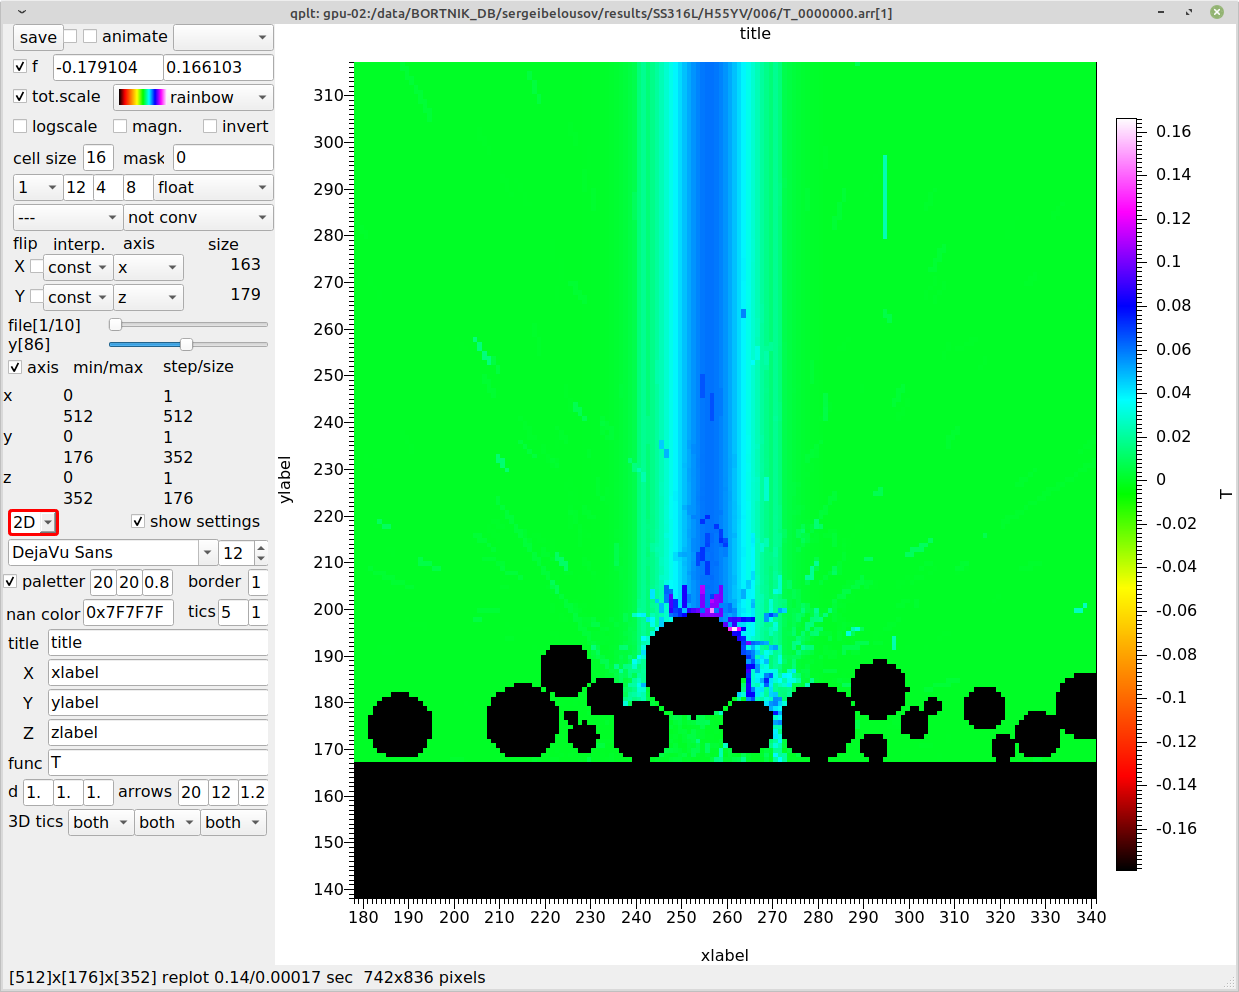
\epsfig{file=picts/2D, width=.7\textwidth} 
      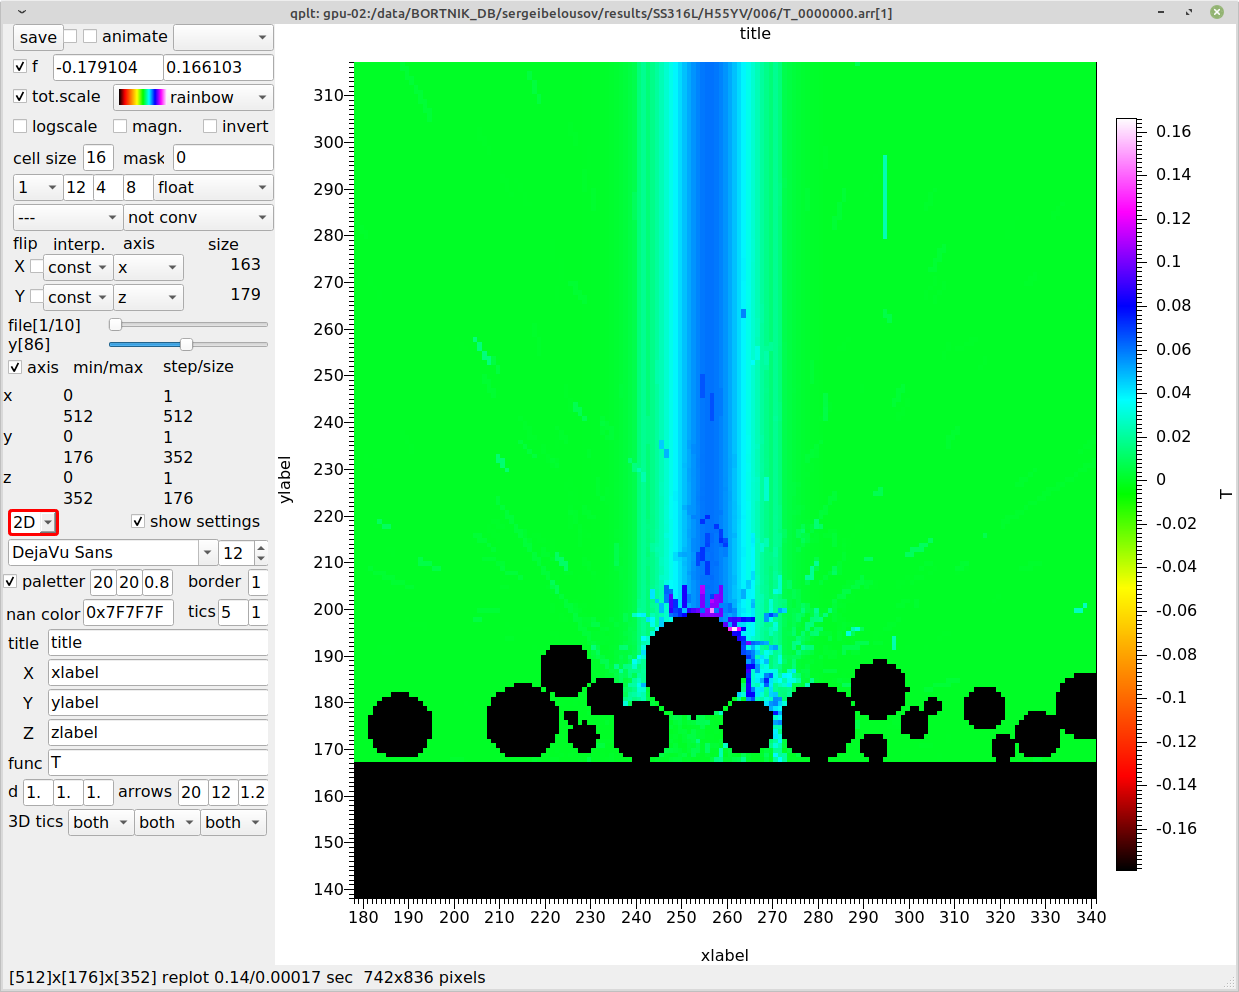
\includegraphics[width=.7\textwidth]{picts/2D.png} 
  \end{center}
  \caption{Режим отображения 2D}\label{2D:pict}
\end{figure}

\begin{figure}
  \begin{center}
      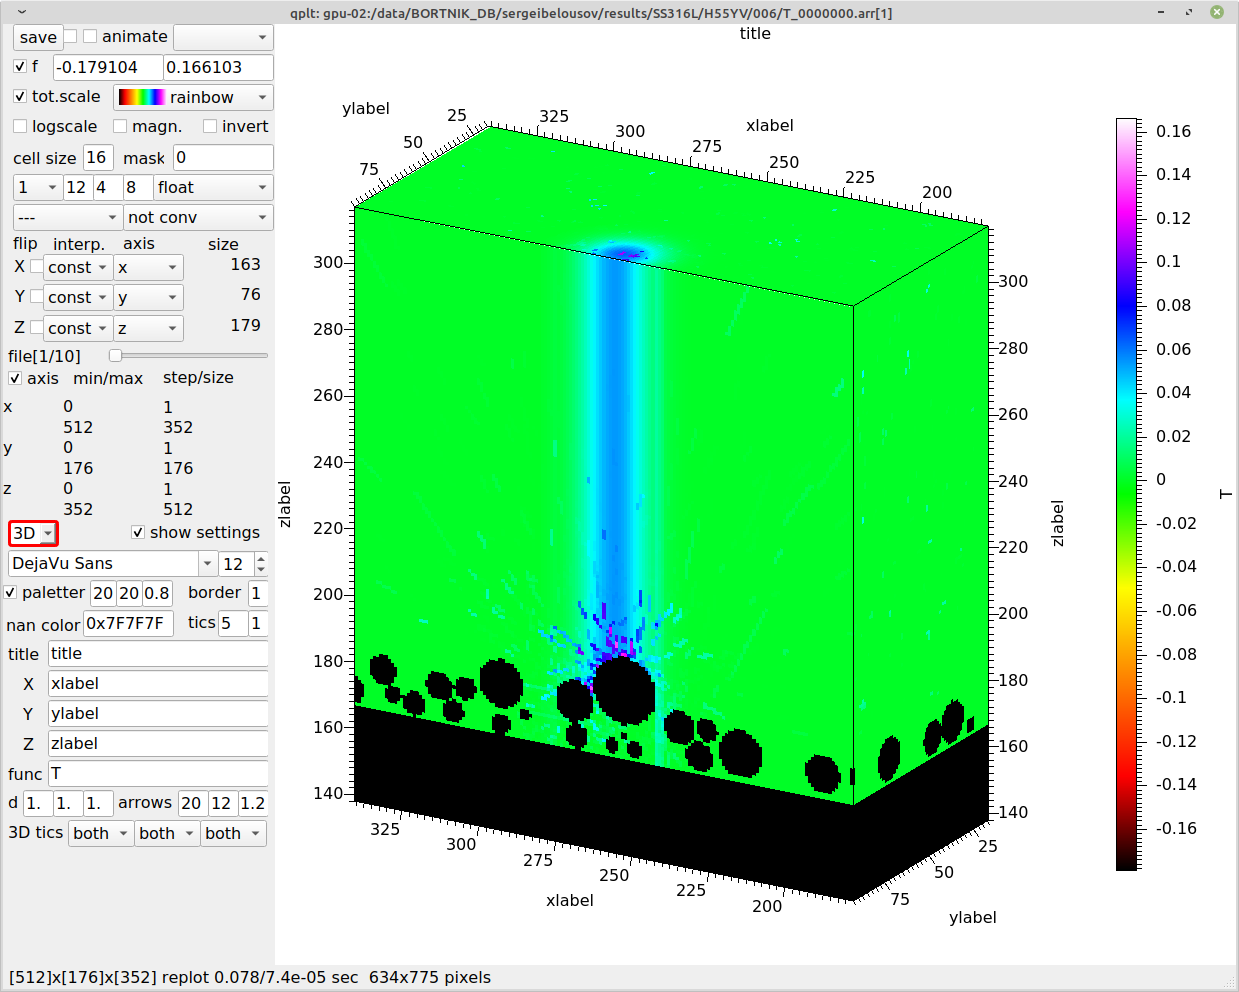
\includegraphics[width=.7\textwidth]{picts/3D.png} 
  \end{center}
  \caption{Режим отображения 2D}\label{3D:pict}
  \begin{center}
      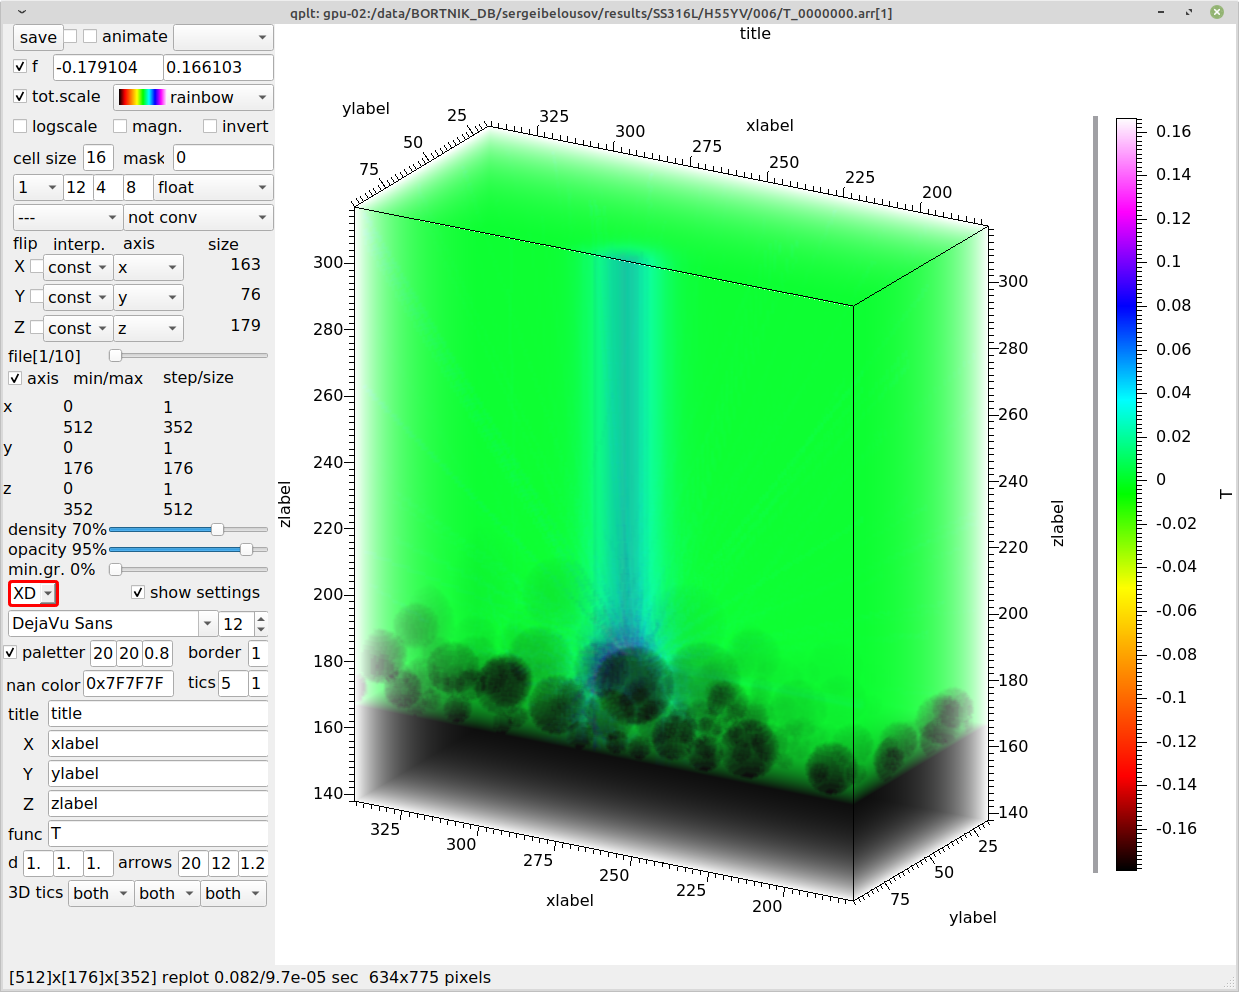
\includegraphics[width=.7\textwidth]{picts/XD.png} 
  \end{center}
  \caption{Режим отображения XD}\label{XD:pict}
\end{figure}
Графический интерфейс представлен одним окном. Слева на узкой вертикальной панели сгруппированы элементы настройки и управления.
Активный элемент управления (на который указывает фокус ввода) выделен красной рамкой.
Основная часть окна отдана для демонстрации изображения. В правой части изображения вертикально размещается палитра. 

Существует три режима отображения~--- двумерный (2D, срез ортогональный главным осям, рис.~\ref{2D:pict}), псевдо-трехмерный (3D, показываются внешние грани куба, рис.~\ref{3D:pict})
и трехмерный (XD, лучи трассируются внутрь куба, рис.~\ref{XD:pict}).

При помощи элементов на панели управления можно получать информацию об открытом кадре с данными; переключаться между файлами и кадрами в файле;
изменять параметры отображаемого среза, область отображения и диапазон отображаемых значений; настраивать способ отображения данных (выбирать
тип данных и их расположение в ячейке, применять к данным различные операции); выбирать оси для отображения, включать/выключать режим интерполяции и т.д.

Для поворота изображения, выбора пределов отображения и ряда других действий используется интуитивно понятный интерфейс,
основанный на взаимодействии мыши и изображения.

При переключении между файлами/кадрами/срезами все выбранные параметры отображения по возможности сохраняются.

При движении курсора по изображению показывается значение функции под курсором. 
При движении курсора по палитре показывается значение палитры под курсором. 

\begin{figure}[h]
  \begin{center}
      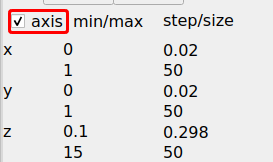
\includegraphics[width=.28\textwidth]{picts/show-axis.png} 
  \end{center}
  \caption{Информация о сетке}\label{show:axis:pict}
\end{figure}
Для вывода информации о сетке служит элемент панели с галочкой \verb'axis' (рис.~\ref{show:axis:pict}).
Если элемент включен, то он отображает по каждой из осей данные о названии оси, пределах, числе ячеек, шаге и логарифмическом масштабе.

Для сохранения изображения служит кнопка \verb'save', поддерживается сохранение в формате \verb'.png'.

Внизу, в строке состояния, показывается размер сетки, время перерисовки и размер изображения, сгенерированного ядром.

\subsection{Настройка входных данных для отображения}
\begin{figure}[h]
  \begin{center}
    \begin{tabular}{lll}
      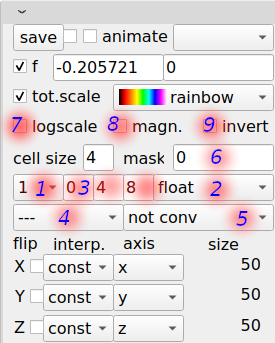
\includegraphics[width=.28\textwidth]{picts/access.png} && 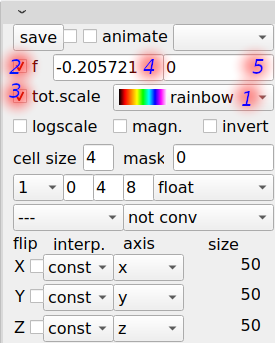
\includegraphics[width=.28\textwidth]{picts/pal.png} \\
      \it а && \it б
    \end{tabular}
  \end{center}
  \caption{Настройка входных данных для отображения ({\it а}) и выбор палитры ({\it б})}\label{access:pict}
\end{figure}


Размер ячейки загруженных данных указан в поле \verb'cell size'. 

При настройке входных данных для отображения необходимо установить (рис.~\ref{access:pict}~{\it а}):
\begin{enumerate}
\item размерность входных данных~--- 1 (по умолчанию), 2 или 3;
\item тип входных данных~--- \verb'float' (по умолчанию), \verb'double', \verb'bool', \verb'uint8_t', \verb'int8_t', \verb'uint16_t', \verb'int16_t', \verb'uint32_t', \verb'int32_t', \verb'uint64_t', \verb'int64_t';
\item смещения в байтах от начала ячейки для каждой из компонент (по умолчанию 0, 4, 8);
\item дифференциальную операцию~--- \verb'---' (не используется, по умолчанию), \verb'div' (дивергенция),
  \verb'grad 2D' (двумерный градиент), \verb'grad 3D' (трехмерный градиент), \verb'rot' (ротор), \verb'laplas 2D' (двумерный оператор Лапласа),
  \verb'laplas 3D' (трехмерный оператор Лапласа);
\item способ приведения полученного вектора к скаляру~--- \verb'X component', \verb'Y component', \verb'Z component', \verb'module', \verb'phase 2D', \verb'not conv'
  (не преобразовывать, по умолчанию);
\item маску (только для целочисленных данных, по умолчанию ноль)~--- позволяет выбирать отдельные биты
  целого числа для отображения;
\item логарифмический масштаб по значению функции;
\item модуль функции;
\item смену знака функции.
\end{enumerate}


\subsection{Выбор палитры  и пределов отображаемой функции}
Существует 10 палитр (рис.~\ref{access:pict}~{\it б, 1}, рис.~\ref{10pals:pict}), расширение набора палитр пользователем не предусмотрено. 

Возможен автоматический выбор пределов функции для отображения (рис.~\ref{access:pict}~{\it б, 2}).
При выборе автоматического режима можно выбирать локальный выбор пределов (для выбранного пространственного фрагмента)
или глобальный выбор пределов по всей области (рис.~\ref{access:pict}~{\it б, 3}). 

Автоматически вычисляемые пределы для заданных параметров отображения вычисляются однократно (это может требовать некоторого времени
для больших массивов) и затем кэшируются ядром для последующего использования.

Пределы отображения указываются в полях ввода (рис.~\ref{access:pict}~{\it б, 3, 4}) и на палитре. Пределы могут задаваться
вручную в виде чисел в полях ввода или при помощи мыши на палитре.

Левая кнопка мыши позволяет выделять на палитре область для отображения.
Щелчок правой кнопки справа от палитры включает режим автоматического выбора пределов или возвращает пределы к последним выбранным вручную значениям.

Колесо мыши может использоваться для зумирования области палитры
(если курсор находится на палитре, при этом рядом с курсором отображается буква \verb'Z') или для прокрутки области отображения (курсор находится справа от палитры).

Щелчок правой кнопкой мыши по палитре используется для включения/выключения прозрачности данного цвета в режиме XD.

\begin{figure}
  \begin{center}
  \begin{tabular}{rl}
    \verb'rainbow' & \framebox{
\includegraphics[width=.8\textwidth, height=5mm]{picts/pals/rainbow.png}} \\
    \verb'positive' & \framebox{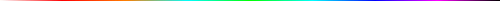
\includegraphics[width=.8\textwidth, height=5mm]{picts/pals/positive.png}} \\
    \verb'neg_pos1' & \framebox{
\includegraphics[width=.8\textwidth, height=5mm]{picts/pals/neg_pos1.png}} \\
    \verb'neg_pos2' & \framebox{
\includegraphics[width=.8\textwidth, height=5mm]{picts/pals/neg_pos2.png}} \\
    \verb'inv_rainbow' & \framebox{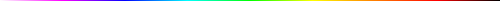
\includegraphics[width=.8\textwidth, height=5mm]{picts/pals/inv_rainbow.png}} \\
    \verb'inv_grey' & \framebox{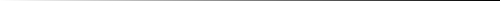
\includegraphics[width=.8\textwidth, height=5mm]{picts/pals/inv_grey.png}} \\
    \verb'grey' & \framebox{
\includegraphics[width=.8\textwidth, height=5mm]{picts/pals/grey.png}} \\
    \verb'green_blue' & \framebox{
\includegraphics[width=.8\textwidth, height=5mm]{picts/pals/green_blue.png}} \\
    \verb'color' & \framebox{
\includegraphics[width=.8\textwidth, height=5mm]{picts/pals/color.png}} \\
    \verb'black_red' & \framebox{
\includegraphics[width=.8\textwidth, height=5mm]{picts/pals/black_red.png}} 
  \end{tabular}
  \end{center}
  \caption{Варианты встроенных палитр qplt}\label{10pals:pict}
\end{figure}


%\pagebreak

\subsection{Выбор отображаемых осей и режимов интерполяции}
\begin{wrapfigure}{r}{.28\textwidth}
  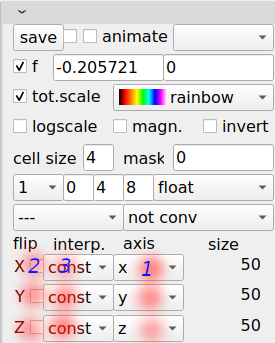
\includegraphics[width=.28\textwidth]{picts/sel-axis.png} 
  \caption{Выбор отображаемых осей и режимов интерполяции}\label{sel:axis:pict}
\end{wrapfigure}
При визуализации сетки размерности $2\div6$ можно выбрать две (или три, в зависмости от режима визуализации)
оси сетки для отображения (рис.~\ref{sel:axis:pict},~{\it 1}). Для каждой из выбранных осей можно независимо задать разворот
(\verb'flip', рис.~\ref{sel:axis:pict},~{\it 2})
и режим интерполяции (рис.~\ref{sel:axis:pict},~{\it 3})~--- \verb'const' (нулевого порядка, по умолчанию),
\verb'linear' (линейная), \verb'cubic' (кубическая), \verb'spline' (кубическим бета-сплайном). 

Кубическая интерполяция обеспечивает точное прохождение интерполянта через узлы табулированной функции, но может приводить к появлению лишних экстремумов между узлами.
Интерполяция кубическим бета-сплайном не обеспечивает точного прохождения интерполянта через узлы табулированной функции,
но не приводит к появлению лишних экстремумов между узлами.

Различные режимы интерполяции работают только в 2D и 3D режимах и не работают в XD режиме.

При переключении осей настройки для каждой из осей сетки сохраняются, то есть режимы разворота и интерполяции привязываются к осям сетки, а не к осям изображения.

\subsection{Выбор файла, кадра и срезов для отображения}
Выбор файла, кадра и срезов для отображения производится при помощи ползунков (слайдеров).
Ползунки показываются по мере необходимости~--- если есть несколько файлов, то ползунок выбора файла показывается всегда;
если в выбранном файле есть несколько кадров, то показывается ползунок выбора кадра;
если для выбранного кадра (и режима отображения) можно выбирать срезы или несколько срезов, то показываются
соответствующие ползунки для выбора срезов.

При переключении файла номер кадра по возможности сохраняется.

Если ползунок выбора среза установлен в ноль, то при переключении файла/кадра показывается первый (по данной оси) срез.
В противном случае запоминается координата среза по заданной оси и отображается ближайший к данной координате срез.

Имя выбраннных файла и кадра отображаются в заголовке окна qplt.

\subsection{Выбор пространственной области для отображения}
В режиме 2D левая кнопка мыши позволяет выбирать пределы отображения как по обоим осям (выделять фрагменты изображения),
так и по одной оси (выделять фрагмент оси). Щелчок правой кнопкой по изображению переключает режим выделения
по обоим осям с автоматического (весь диапазон) на последний диапазон, выбранный вручную. 
Щелчок правой кнопкой по оси (за пределами изображения) переключает режим выделения по данной оси.

В режимах 3D/XD левая кнопка мыши позволяет выделять диапазон отображения по каждой из осей. 
Щелчок правой кнопкой по оси (за пределами изображения) переключает режим выделения по данной оси.
Когда курсор  находится над кубом изображения, левая кнопка позволяет поворачивать куб изображения.
Двойной щелчок за пределами куба изображения разрезает куб изображения пополам по данной оси и оставляет ту половину,
по которой был произведен щелчок. Двойной щелчок по грани куба разворачивает эту грань на пользователя и включает 2D режим.

Во всех режимах, если курсор мыши находится над изображением, то колесо мыши зумирует изображение.
Если курсор мыши находится за пределами изображения, то колесо позволяет либо прокручивать область отображения по данной оси (если курсор
близко к изображению), либо зумировать изображение по данной оси (если курсор далеко от изображения, при этом рядом с курсором отображается буква \verb'Z').

Во всех случаях выбор области отображения квантуется по ячейкам сетки. 
Выбранная область отображения привязана к осям сетки.

При переключении осей настройки пределов отображения для каждой из осей сетки сохраняются, то есть пределы отображения привязываются к осям сетки, а не к осям изображения.

При переключении файлов/кадров выбранная область отображения сохраняется не в номерах ячеек, а в абсолютной системе координат.
Размер выбранной области отображения в ячейках показывается на панели управления около элементов выбора осей для отображения.

\subsection{Трехмерный рендеринг}
При трехмерном рендеринге (режим XD) появляются дополнительные настройки отображения~--- прозрачность узловых цветов палитры,
плотность (density), суммарная прозрачность (opacity) и порог градиента (min.gr).

Профиль прозрачность узловых цветов палитры отображается в виде серой линии слева от палитры. По умолчанию все цвета считаются непрозрачными.
Щелчок правой кнопки мыши по палитре включает/выключает прозрачность цвета. Число узловых цветов зависит от палитры.

Плотность задает глубину, на которую трассируемые из плоскости экрана лучи проникают вглубь сетки. Нулевая плотность
делает сетку прозрачной на всю глубину, 100\% плотность эквивалентна режиму 3D.

Суммарная прозрачность показывает, насколько итоговое изображение будет прозрачным после того, как луч проник на максимально возможную глубину.

\begin{figure}[hb]
  \begin{center}
      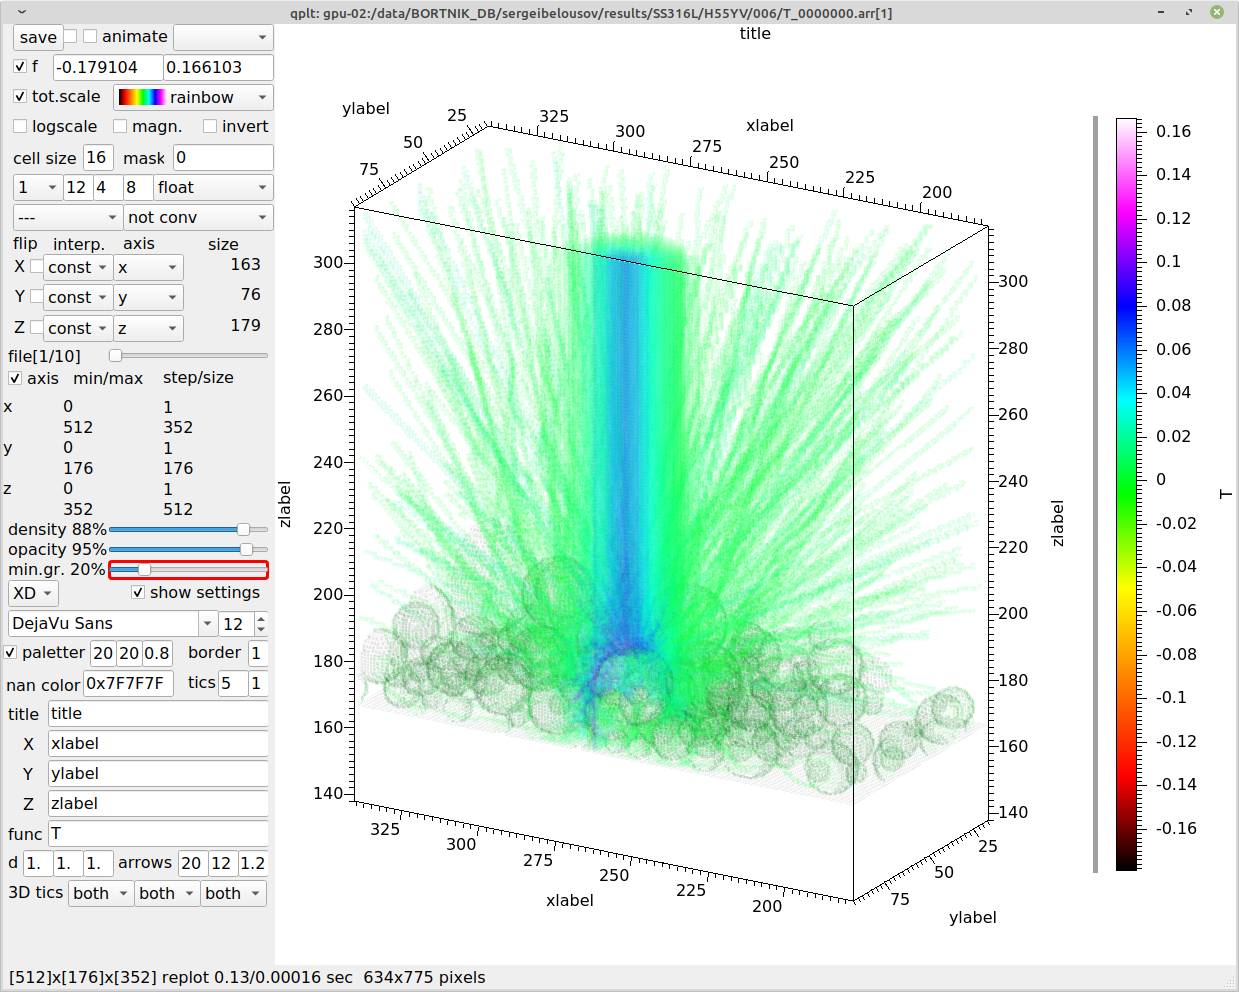
\includegraphics[width=.7\textwidth]{picts/XD-grad.png} 
  \end{center}
  \caption{Режим отображения XD с отсечкой по минимальному градиенту вдоль луча}\label{XD:grad:pict}
\end{figure}

Минимальный градиент задает (в логарифмической шкале) некоторое минимальное значение градиента вдоль луча, ниже которого значение считается прозрачным, рис.~\ref{XD:grad:pict}.

\subsection{Визуализация векторных полей}
\begin{figure}[h]
  \begin{center}
      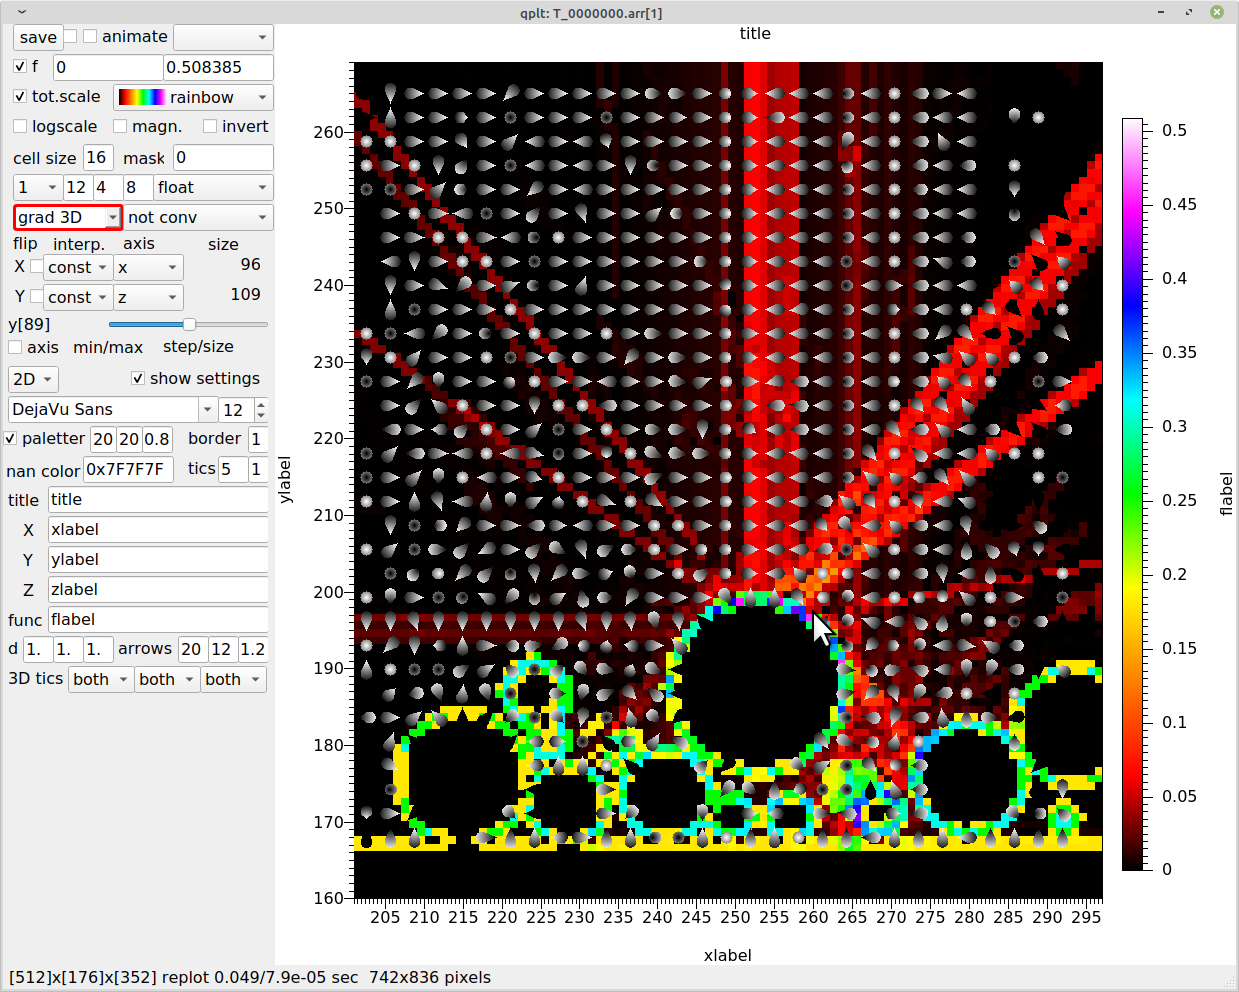
\includegraphics[width=.7\textwidth]{picts/2D-grad.png} 
  \end{center}
  \caption{Визуализация векторных полей}\label{2D:grad:pict}
\end{figure}
Визуализация векторных полей поддерживается только в 2D режиме.
В 3D/XD режимах визуализируется модуль векторного поля. 

В 2D режиме поверх векторного поля рисуется равномерная сетка из конусов в градациях серого, рис.~\ref{2D:grad:pict}.
Каждый конус отвечает нормали (единичному вектору направления) векторного поля.
Вершина конуса указывает направление вектора в плоскости
изображения, по длине конуса можно оценить, насколько вектор выходит из плоскости изображения.

Ориентацию вектора ортогонально плоскости изображения (наружу/вглубь экрана) можно оценить по тональной перспективе~---
ближайшая часть конуса окрашена в более темный цвет.


\subsection{Дополнительные настройки отображения}
\begin{figure}[h]
  \begin{center}
      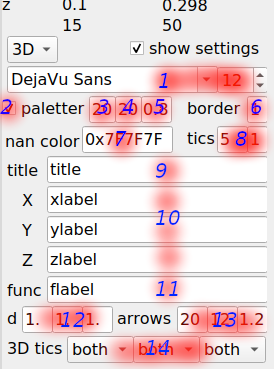
\includegraphics[width=.28\textwidth]{picts/settings.png} 
  \end{center}
  \caption{Дополнительные настройки отображения}\label{settings:pict}
\end{figure}
Дополнительные настройки можно показать/скрыть на панели слева при помощи галочки \verb'show settings' (рис.~\ref{settings:pict}).
Дополнительные настройки включают в себя

\begin{enumrate}
\item настройки шрифта зарамочного оформления;
\item включение/выключение показа палитры;
\item расстояние между палитрой и изображением в пикселях;
\item ширину палитры в пикселях;
\item высоту палитры (доля от высоты окна);
\item ширину рамок в пикселях;
\item цвет, которым задаются значения \verb'nan';
\item длину и толщину тиков на подписях к осям (тики напротив которых стоят числа будут  вдвое длиннее);
\item заголовок изображения;
\item подписи к осям изображения;
\item подпись к палитре;
\item соотношение сторон ячейки в 3D/XD режимах;
\item длину и ширину конусов, а также шаг конусов при отображении векторных полей в 2D режиме;
\item правила расстановки тиков и подписей к осям в 3D/XD режимах.
\end{enumerate}


Заголовок изображения форматируется по словарю файла, получаемого в случае загрузки данных из \verb'json' с опцией \verb'-f'.
Это позволяет автоматически выводить в заголовок различные параметры, связанные с файлом. Для форматирования используется
метод \verb'str.format' языка \verb'Python3'.

Метки к осям привязаны к осям изображения, а не осям сетки, и не переключаются при смене осей сетки.

Для расстановки тиков и подписей к осям в 3D/XD режимах возможны следующие варианты (каждая ось обрабатывается независимо):
\begin{itemize}
\item \verb'both' --- тики и подписи выводятся с обеих сторон куба изображения;
\item \verb'auto' --- тики выводятся с обеих сторон куба изображения, подпись выводится слева/внизу;
\item \verb'up/down' (для оси Z \verb'left/right') --- тики и подпись выводятся с одной стороны куба изображения;
\item \verb'off' --- тики и подпись для данной оси отключены.  
\end{itemize}
%%%%%%%%%%%%%%%%%%%%%%%%%%%%%%%%%%%%%%%%%%%%%%%%%%%%%%%%%%%
\section{Форматы данных}
Могут визуализироваться данные размерности $2\div6$ заданные на равномерной прямоугольной сетке.
В библиотеке \verb'aiwlib' такие сетки реализованы в виде класса \verb'Mesh<typename T, int D>'. 

%\begin{table}
\begin{center}
\begin{tabular}{|p{.1\textwidth}|p{.25\textwidth}|p{.21\textwidth}|p{.35\textwidth}|}
\hline
величина & длина, байт & тип & описание величины \\
\hline
\multicolumn{4}{|c|}{заголовок \rule{0pt}{.6cm}}\\
\hline
{\tt h\_sz} & {\tt 4} & {\tt uin32\_t} & длина текстового заголовка \\
{\tt h} & {\tt h\_sz*4} & {\tt char*} & текстовый заголовок \\
{\tt D} & {\tt 4} & {\tt uint32\_t} & размерность сетки\\
{\tt szT} & {\tt 4} & {\tt uint32\_t} & размер ячейки сетки в байтах\\
{\tt box} & {\tt D*4} & {\tt uint32\_t[D]} & размеры сетки в ячейках\\
\hline
\multicolumn{4}{|c|}{данныe \rule{0pt}{.6cm}}\\
\hline
{\tt data} & {\tt szT*box[0]*box[1]*...} & пользовательский & ось $x$ самая быстрая \\
\hline
\end{tabular}
\end{center}
% \end{table}

Опционально, в {\bf текстовый} заголовок могут быть записаны следующие данные (размещаются после первого нулевого байта {\tt h})
\begin{center}
\begin{tabular}{|p{.1\textwidth}|p{.12\textwidth}|p{.21\textwidth}|p{.48\textwidth}|}
\hline
величина & длина, байт & тип & описание величины \\
\hline
  {\tt axis} & --- & {\tt char*[D]} & имена осей сетки записываются последовательно, каждая ось состоит из длины (четырехбайтовое целое) и, собственно, имени\\
  {\tt typeinfo} & --- & {\tt aiw::TypeInfo} & описание структуры ячейки сетки в настоящий момент не поддерживается \\
  {\tt out\_value} & {\tt szT} & пользовательский & значение на бесконечности (за пределами сетки) \\
  {\tt align} & --- & --- & некоторое количество нулей, необходимое для выравнивания данных сетки на 64 байта \\
  {\tt bmin} & {\tt D*8} & {\tt double[D]} & координаты левого нижнего угла сетки \\
  {\tt bmax} & {\tt D*8} & {\tt double[D]} & координаты правого верхнего угла сетки \\
  {\tt mask} & {\tt 4} & {\tt uint32\_t} & битовая маска \\  
  \hline
\end{tabular}
\end{center}
Битовая маска содержит:
\begin{itemize}
  \item 31-й бит --- флаг наличия имен осей;
  \item 30-й бит --- флаг наличия структуры {\tt TypeInfo};
  \item младшие биты --- флаги логарифмического масштаба по соответствующим осям.
\end{itemize}
%%%%%%%%%%%%%%%%%%%%%%%%%%%%%%%%%%%%%%%%%%%%%%%%%%%%%%%%%%%
\section{Информационные сообщения и сообщения об ошибках}  
\subsection{Сообщения при запуске}
\verb'File ~/.ssh/config not loaded' --- возникли какие-то сложности с загрузкой файла \verb'~/.ssh/config'.
Это не является ошибкой, но может означать для OS Linux, что короткие имена для удаленных машин окажутся недоступными в клиент-серверном режиме работы.

\verb'Module qplt.core is not available' --- не удалось загрузить локальную версию ядра. Это не является ошибкой, но визуализация локальных файлов с данными будет недоступна.

\verb'Module qplt.remote is not available' --- не удалось загрузить модуль для удаленного запуска ядер визуализации (скорее всего, не установлен пакет \verb'paramiko').
Это не является ошибкой, но удаленная визуализация файлов с данными будет недоступна.

\verb'Load [ <filename> ] --- skipped' --- файл с именем \verb'<filename>' пропущен. Это не является ошибкой.
Скорее всего, файл не существует, пустой или содержит данные в нераспознанном формате (из файла не удалось загрузить ни одного кадра с данными). 

\verb'Module qplt.core is not imported, local file [ <filename> ] skipped' --- поскольку локальная версия ядра недоступна,
файл с именем \verb'<filename>' пропущен. Это не является ошибкой.

\verb'Module qplt.remote is not imported, file [ <filename> ] by connect <host> skipped' --- поскольку модуль для работы с удаленными ядрами недоступен,
файл с именем \verb'<filename>'  на сервере \verb'<host>' пропущен. Это не является ошибкой.

\verb'... --- skipped incorrect mem_limit argumet -m...' --- пропущен неверный аргумент, задающий лимит памяти. Скорее всего, строка после \verb'-m'
не может быть приведена к типу \verb'float'. Это не является фатальной ошибкой.

\verb'Load <file> --- <count> frames' --- из файла \verb'<file>' загружено \verb'<count>' кадров с данными.

\verb'Totally loaded <count> frames from <fcount> files' --- суммарно загружено \verb'<count>' кадров с данными из \verb'<fcount>' файлов. Это итоговое сообщение,
выводимое после обработки всех файлов с данными.

\subsection{Сообщения во время работы}
\verb|Can't format title ...| --- не удается сформировать заголовок изображения. Скорее всего, в тексте заголовка есть ошибки с точки зрения фукции \verb'str.format'.
Сообщения о возникших проблемах выводятся в том же сообщении. Это не является фатальной ошибкой, но заголовок изображения будет некорректным.

Для всех полей ввода, принимающих числа, при вводе проводится проверка введенного значения. Если введенное значение некорректно, выводится сообщение
о возникших проблемах и используется последнее корректное введенное значение.

При возникновении фатальной ошибки в консоль выводится стек исключения \verb'python',
после чего выводится сообщение
\begin{verbatim}
#
#>>>  <file>[<frame>]
#
\end{verbatim}
где \verb'<file>' --- имя файла, \verb'<frame>' --- номер кадра с данными из файла для которых возникла ошибка.
При этом приложение завершает свою работу.
В этом случае необходимо обратиться к разработчику, приложив выводы стека исключения
и, желательно, файл с данными, в котором возникла проблема.

Возможны сообщения об ошибках
\begin{verbatim}
src/qplt/mesh_cu.cpp data_load_impl():28 can't allocate memory in device (size=<size>, err=<err>)
src/qplt/mesh_cu.cpp plot():124 can't allocate memory in device (size=<size>, err=<err>)
\end{verbatim}
которые могут возникать в ядре, собранном с поддержкой GPU. Сообщения означают, что не удалось выделить на видеокарте память размера \verb'<size>'
и функция \verb'cudacudaMalloc()' вернула ошибку с кодом \verb'<err>'. При этом приложение завершает свою работу.
В этом случае следует обратиться к разработчику. Если ошибка возникает слишком часто, используйте сборку qplt без поддержки GPU.

В случае, если ошибка произошла в ядре визуализации, запущенном удаленно, на хосте \verb'<host>' выводится сообщение
\begin{verbatim}
RECV <host> FAILED:
\end{verbatim}
после чего следует вывод из стандартного потока ошибок ядра. При этом приложение завершает свою работу.

\subsection{Сообщения при завершении работы}
Для каждого ядра визуализации, запущенного удаленно, на хосте \verb'<host>' при завершении работы выводится сообщение
\begin{verbatim}
FINAL REPORT <host>:
\end{verbatim}
после чего следует вывод из стандартного потока ошибок ядра визуализации. 

%%%%%%%%%%%%%%%%%%%%%%%%%%%%%%%%%%%%%%%%%%%%%%%%%%%%%%%%%%%
\section{Алгоритмы визуализации}
При загрузке файлов для каждого кадра с данными считываются размерность кадра (от двух до шести), размер ячейки сетки в байтах, размеры сетки в ячейках
и пределы сетки по осям в некоторой глобальной системе координат. При этом определяется положение блока данных в файле, но реального считывания данных не происходит.

При визуализации данные подгружаются в память менеджером памяти. Если ядро визуализации собрано с поддежкой GPU,
память выделяется командой \verb'cudaMallocManaged' и затем данные копируются из файла. Если ядро собрано без поддежки GPU,
под OS Linux данные мапируются из файла в память, для OS Windows память выделяется командой \verb'new', и затем данные копируются из файла.
Ранее загруженные, но не используемые данные могут быть выгружены из памяти, если суммарный размер памяти, выделенной под данные, превышает заданный лимит памяти.
За загрузку/выгрузку данных отвечает менеджер памяти, реализованный в классе \verb'QpltContainer'.

После загрузки данных создается плоттер~--- экземпляр класса, наследующий базовый класс \verb'QpltPlotter'.
При создании плоттер  получает все параметры отрисовки (ориентацию куба изображения, набор осей, пределы по осям и т.д.) кроме размера изображения.
Если включено автошкалирование по значению функции, то определяются (или загружаются из кэша) пределы отрисовки функции.
Плоттер создает в т.ч. набор флэтов (экземплятров класса \verb'QpltFlat'), описывающий
грани куба изображения, развернутые на пользователя.

Далее рисуется заголовок изображения. Определется расстановка тиков вдоль палитры, определяется отступ палитры от правого края и рисуется палитра.
После этого для плоттера вызывается метод \verb'set_image_size', устанавливающий координаты вершин флэтов в пикселях.
Производится оценка расстановки тиков, и размер изображения корректируется так, чтобы тики и подписи к осям не выходили
за пределы окна и не накладывались друг на друга. Снова вызывается метод \verb'set_image_size', корректирующий размеры
изображения, и, наконец, вызывается метод \verb'plot()', генерирующий изображение в виде строки. Изображение выводится на экран,
поверх изображения рисуются оси, тики и подписи к осям.

В начале метода \verb'plot' для каждого флэта генерируется объект, обеспечивающий доступ к данным. Объект хранит указатель на ячейку данных, попадающую в угол флэта,
расстояния в байтах для смещения по каждой из осей и предоставляет функции перехода из экранных координат в координаты флэта (в ячейках).

Если ядро собрано без поддержки GPU, то метод \verb'plot()' обходит все пиксели в двойном цикле по $x, y$, цикл по $у$
является внешним и распараллеливается средствами OpenMP. В цикле определяется флэт, на который попадает пиксель, а затем происходит вычисление цвета пикселя.
Если ядро собрано  с поддержкой GPU, то для каждого пикселя изображения запускается свое ядро GPU, вычисляющее цвет пикселя.

В режимах 2D/3D цвет пикселя определяется на основе значения в ячейке флэта, в которую проецируются пиксель и палитры,
при этом может предварительно производиться интерполяция значения. В режиме XD для каждого пикселя генерируется экземпляр
класса \verb'VTexture'. Этот объект обеспечивает аналитическое решение задачи о пересечении луча и вкоселя. При этом вычисляется длина фрагмента луча,
грань, через которую луч выходит из вокселя, и экземпляр класса \verb'VTexture' перенастраивается для обработки следующего вокселя, в который попадает луч.
Для каждого фрагмента луча, проходящего через воксель, на основе значения в вокселе определяется цвет луча. Полученное значение подсуммируется 
в цвет пикселя с учетом длины фрагмента луча, прозрачности и градиента функции вдоль луча. 


%%%%%%%%%%%%%%%%%%%%%%%%%%%%%%%%%%%%%%%%%%%%%%%%%%%%%%%%%%%
\section{Информация о файлах с исходным кодом}   %1
Пути ко всем файлам показаны от корня директории, содержащей библиотеку aiwlib.
\subsection{Исполняемые файлы}
Файл \verb'bin/qplt' содержит головной скрипт на языке \verb'python', реализующий графический интерфейс и вызывающий основные функции визуализации.

Файл \verb'src/bin/qplt-remote.cpp' содержит функцию \verb'main()' для запускаемого удаленно ядра визуализации.

\subsection{Модули python}
Файл \verb'python3/aiwlib/qplt/factory.py' импортирует ядра визуализации, содержит классы и методы для разбора аргументов командной строки,
запускает загрузку файлов с данными в ядрах визуализации.

Файл \verb'python3/aiwlib/qplt/remote.py' содержит код для работы с запускаемыми удаленно ядрами визуализации.

Файл \verb'python3/aiwlib/qplt/canvas.py' содержит код класса \verb'Canvas', отвечающий за графический интерфейс, построение изображения и его
зарамочное оформление.

Файл \verb'python3/aiwlib/qplt/mouse.py' содержит код, реализующий обработку событий мыши.

Файл \verb'python3/aiwlib/qplt/tics.py' содержит код для расстановки тиков вдоль осей.

\subsection{Модули C++}

Файлы \verb'src/qplt/base.cpp' и \verb'aiwlib/include/qplt/base' содежат код базовых классов \verb'QpltContainer',
\verb'QpltPlotter', \verb'QpltFlat' и функции \verb'qplt_global_init()', \verb'std::vector<QpltContainer*> factory(const char *fname)'.
Файл \verb'aiwlib/include/qplt/base' обрабатывается утилитой \verb'swig' и полностью реализует интерфейс локального ядра визуализации. 

Файлы \verb'src/qplt/imaging.cpp' и \verb'aiwlib/include/qplt/imaging' реализуют работу с палитрой (превращение значения типа \verb'float' в цвет),
отрисовку конусов для визуализации векторных полей и генерацию изображения в формате \verb'.ppm'.

Файлы \verb'src/qplt/accessor.cpp' и \verb'aiwlib/include/qplt/accessor' реализуют обработку одной ячейки данных сетки~--- преобразование
встроенных типов во \verb'float', дифференциальные операторы и их дальнейшую обработку. 

Файлы \verb'src/qplt/mesh.cpp' и \verb'aiwlib/include/qplt/mesh' реализуют загрузку данных в формате \verb'aiw::Mesh',
расчет пределов и реализации всех необходимых классов визуализации. 

Файлы \verb'src/qplt/mesh_cu.cpp' и \verb'aiwlib/include/qplt/mesh_cu' реализуют рендеринг лучей в режиме XD.

Файлы \verb'src/qplt/vtexture.cpp' и \verb'aiwlib/include/qplt/vtexture' содержат код класса VTexture необходимый для рендеринга лучей в режиме XD.

При сборке с поддежкой GPU модуль \verb'src/qplt/mesh_cu.cpp' компилируется не \verb'g++', а \verb'nvcc', компоновка кода так же осуществляется
при помощи \verb'nvcc'. 

\subsection{Модули C++ из ядра библиотеки aiwlib}
Файлы \verb'include/aiwlib/debug' и \verb'src/debug.cpp' содержат код для обработки ошибок и вывода различных сообщений.

Файл \verb'include/aiwlib/alloc' содержит код мапирования файлов в память.

Файл \verb'include/aiwlib/interpolate' содержит алгоритмы интерполяции.

Файлы \verb'include/aiwlib/iostream' и \verb'include/aiwlib/binaryio' работу с файлами и ввод/вывод в бинарном формате.

Файлы \verb'include/aiwlib/binary_format' и \verb'src/binary_foramt.cpp' реализуют чтение заголовков файлов с данными в формате \verb'aiw::Mesh'.

Файлы \verb'include/aiwlib/vec' и \verb'include/aiwlib/matr' реализуют линейную алгебру (вектора и матрицы), необходимую в т.ч. для визуализации.


\subsection{Дополнительные файлы}
Файл \verb'python3/aiwlib/qplt/qplt.ui' содержит внешний вид графичекого интерфейса, нарисованного в QtDesigner.

Файлы \verb'python3/aiwlib/qplt/pals/*.ppm' содержат палитры.

Файл \verb'python3/aiwlib/qplt/pals/size' содержит размеры палитры (число узловых цветов).


\end{document}
